\newpage
\section{Evaluation}
\label{sec:evaluation}

To estimate the obtained C2 Maneuver Agility in the system, we collected evidence from the implementation based on the proposed model. Such simulation plays different scenarios that explore dynamic contexts, i.e.., the circumstances can change during the mission execution. These scenarios allow us to test the system effectiveness under such conditions applying the C2 concept. Thus, our goal with the simulations is to answer the following research question:

\begin{center}
\fbox{\begin{minipage}{25em}
\textit{How the C2 Maneuver Agility contributes with the C2 Agility?}
\end{minipage}}    
\end{center}

Next, we define the metrics applied in the evaluation to answer the proposed question and their corresponding descriptions:
\begin{itemize}
    \item Maneuvering (M1): Number of C2 Maneuvers performed by the members to accomplish the mission within a given timeout;
    \item Timeliness (M2): System time, in ticks, to accomplish the mission within a given timeout;
    \item Effectiveness (M3): Percentage of successful tasks completed by the executors.
\end{itemize}

We applied two different methods of response in case of context changes, so-called A1 and A2. Both methods starts the execution with an initial context predefined and it performs a task allocation. To the A1 method, the context changes, e.g., member dropped, or sensors' issue, does not initiate any system's reaction to deal with. In such case, the system just keeps running and can become ineffective with the new circumstance. In turn, the A2 method applies the C2 Agility concept to deal with these new conditions. This strategy includes the C2 Maneuver Agility represented by the computational model proposed in Section~\ref{sec:channelSystem} and whose implementation is described in Section~\ref{sec:design}.

The simulation based on an agent tool incorporates C2 Agility characteristics in face of the events created to simulate a dynamic scenario. According to this architecture, C2 Maneuver Agility looks for a suitable adoption of the communication structure to provide an information exchanging, which increases member's awareness. Such coordination structure, represented by the network topology played by the members, is relevant to the members get a suitable task allocation and reconfiguration, i.e., enabling and disabling its sensors in runtime. Thus, the A2 method applies both behaviors, i.e., C2 Agility, in response to new circumstances in the scenarios.

%%%%%%%%%%%%%%%%%%%%%%%%%%%%%%%%%%
% SUBSECTION 
%%%%%%%%%%%%%%%%%%%%%%%%%%%%%%%%%%
\subsection{Simulation Scenarios}
\label{sub:scenarios}

A simulation scenario is composed of an initial context and a sequence of events that provide dynamism. The initial context comprises the set $E$ of members operating an initial C2 Approach $\omega$, the mission $M$ composed of a set of tasks, and the environment. Each possible event, e.g., \textit{memberFailure}, \textit{sensorFailure}, and \textit{envChange}, represents an action that causes a member or environment changes in runtime. These actions are called during simulation to create a dynamic scenario, resembling realistic settings.

The environment represents all the conditions of the place where the members act, e.g., weather conditions, hazard, and communication restrictions. Onboard sensors' capability alteration represents such changes. Based on this, a foggy or cloudy day reduces the uselessness of VGA cameras depending on the task to be performed. Thus, all members with this type of sensors are impacted and it modifies the task allocation performed.

Table \ref{tab:scenarios} shows the sequences of actions that characterizes the context changes in dynamic scenarios. These sequences combined with the same initial context, i.e., members, mission, environment, and the initial C2 Approach,  define the scenarios manipulated by the simulation. These scenarios have a time limit of execution, and the events of environment changes follow the sequences showed. However, their turn is randomly within the simulation timeout.  

\begin{table}[h]
\centenring
\fontsize{9}{9}
\selectfont
\caption{List of events(\textit{EC-envChange; SF-sensorFailure; MF-memberFailure}) that characterizes the context changes within the scenarios tested. The initial C2 Approach, the set of members $E$ and the mission $M$ remain unchanged.}
\label{tab:scenarios}
\begin{tabular}{|m{0.1\textwidth}|m{0.84\textwidth}|}
\hline
\rowcolor{lightgray}
 \textbf {Scenario} & \hfil  \textbf {Context Changes} \\
\hline
 \hfil 1 & EC $\rightarrow$ EC $\rightarrow$ EC $\rightarrow$ EC $\rightarrow$ EC\\
\hline 
 \hfil 2 & EC $\rightarrow$ EC $\rightarrow$ EC $\rightarrow$ EC $\rightarrow$ EC $\rightarrow$ EC $\rightarrow$ EC $\rightarrow$ EC $\rightarrow$ EC $\rightarrow$ EC $\rightarrow$ EC $\rightarrow$ EC $\rightarrow$ EC $\rightarrow$ EC $\rightarrow$ EC \\
\hline 
 \hfil 3 & 
EC $\rightarrow$ EC $\rightarrow$ EC $\rightarrow$ EC $\rightarrow$ EC $\rightarrow$ MF $\rightarrow$ EC $\rightarrow$ EC $\rightarrow$ EC $\rightarrow$ EC $\rightarrow$ EC $\rightarrow$ MF $\rightarrow$ EC $\rightarrow$ EC $\rightarrow$ EC $\rightarrow$ EC $\rightarrow$ EC $\rightarrow$ MF $\rightarrow$ EC $\rightarrow$ EC $\rightarrow$ EC $\rightarrow$ EC $\rightarrow$ EC  \\
\hline 
 \hfil 4 & EC $\rightarrow$ EC $\rightarrow$ EC $\rightarrow$ EC $\rightarrow$ EC $\rightarrow$ SF $\rightarrow$ EC $\rightarrow$ EC $\rightarrow$ EC $\rightarrow$ EC $\rightarrow$ EC $\rightarrow$ SF $\rightarrow$ EC $\rightarrow$ EC $\rightarrow$ EC $\rightarrow$ EC $\rightarrow$ EC $\rightarrow$ SF $\rightarrow$ EC $\rightarrow$ EC $\rightarrow$ EC $\rightarrow$ EC $\rightarrow$ EC  \\
\hline 
 \hfil 5 & EC $\rightarrow$ EC $\rightarrow$ EC $\rightarrow$ SF $\rightarrow$ EC $\rightarrow$ EC $\rightarrow$ EC $\rightarrow$ MF $\rightarrow$ EC $\rightarrow$ EC $\rightarrow$ EC $\rightarrow$ SF $\rightarrow$ EC $\rightarrow$ EC $\rightarrow$ EC $\rightarrow$ MF $\rightarrow$ EC $\rightarrow$ EC $\rightarrow$ EC $\rightarrow$ SF $\rightarrow$ EC $\rightarrow$ EC $\rightarrow$ EC $\rightarrow$ MF  \\
\hline 
 \hfil 6 & EC $\rightarrow$ SF $\rightarrow$ MF $\rightarrow$ EC $\rightarrow$ SF $\rightarrow$ EC $\rightarrow$ SF $\rightarrow$ EC $\rightarrow$ SF $\rightarrow$ MF $\rightarrow$ EC $\rightarrow$ SF $\rightarrow$ EC $\rightarrow$ SF $\rightarrow$ EC $\rightarrow$ SF \\
\hline 
 \hfil 7 & MF $\rightarrow$ SF $\rightarrow$ EC $\rightarrow$ EC $\rightarrow$ EC $\rightarrow$ EC $\rightarrow$ EC $\rightarrow$ EC $\rightarrow$ EC $\rightarrow$ EC $\rightarrow$ EC $\rightarrow$ EC $\rightarrow$ MF $\rightarrow$ SF $\rightarrow$ EC $\rightarrow$ EC $\rightarrow$ EC $\rightarrow$ EC $\rightarrow$ EC $\rightarrow$ MF $\rightarrow$ SF $\rightarrow$ EC $\rightarrow$ EC $\rightarrow$ EC $\rightarrow$ MF $\rightarrow$ SF $\rightarrow$ EC \\
 \hline
 \hfil 8 & MF $\rightarrow$ SF $\rightarrow$ EC $\rightarrow$ MF $\rightarrow$ SF $\rightarrow$ EC $\rightarrow$ MF $\rightarrow$ SF $\rightarrow$ EC $\rightarrow$ MF $\rightarrow$ SF $\rightarrow$ EC \\
 \hline
 \hfil 9 & SF $\rightarrow$ SF $\rightarrow$ SF $\rightarrow$ MF $\rightarrow$ SF $\rightarrow$ SF $\rightarrow$ SF $\rightarrow$ MF $\rightarrow$ SF $\rightarrow$ SF $\rightarrow$ SF $\rightarrow$ MF $\rightarrow$ SF $\rightarrow$ SF $\rightarrow$ SF \\
 \hline
 \hfil 10 & SF $\rightarrow$ EC $\rightarrow$ MF $\rightarrow$ SF $\rightarrow$ EC $\rightarrow$ MF $\rightarrow$ SF $\rightarrow$ EC $\rightarrow$ MF $\rightarrow$ SF $\rightarrow$ EC $\rightarrow$ MF $\rightarrow$ EC $\rightarrow$ EC $\rightarrow$ EC $\rightarrow$ EC $\rightarrow$ EC $\rightarrow$ EC $\rightarrow$ EC $\rightarrow$ EC $\rightarrow$ EC $\rightarrow$ EC \\
 \hline
\end{tabular}

\end{table}


The simulation operates a scenario with 5 possible types of tasks (0 to 4) and 5 types of sensors (A, B, C, D, and E). The tasks and sensors onboard are randomly chosen before the running round. When the tasks allocation process starts, the algorithm applies a function that returns the quality $Q_{ij}$, obtained from a table, that correlates a sensor $i$ to the task $j$. When $Q_{ij}=0$ it means the sensor $i$ is not able to perform the task $j$.

A context change simulated by the system causes the quality reduction of a specific type of sensor, e.g., an environment change simulating a luminosity decreasing reduces in $50\%$ the quality of the sensor type 2 that represents a VGA camera. In case the sensor burns out, its quality comes to be zero and the task will be transmitted to another member to check its execution capacity. Also, the member with a burned sensor is capable of enabling and disabling sensors depending on the task it is currently executing. For instance, after the quality reduction of its sensor type 2, it disables the defective sensor while enabling the best sensor for its next target, present in its allocation list. Furthermore, we can lose a member and, consequently, all its sensors onboard.

Context changes can generate situations such as the tasks reallocation is not enough to keep mission execution. In that case, the C2 System performs a C2 Approach change, i.e.., maneuvering. The new C2 Approach operated can provide a higher awareness level, i.e.., more information shared by the members with a new communication structure, and it can help the members perform reallocation based on the new data exchanged. The initial C2 Approach for all scenarios simulated is De-Conflicted, i.e., a ring communication structure. From this C2 Approach, the maneuver follows incrementally over a specific order of C2 Approaches, based on the following research~\cite{france2014}, and going back to Conflicted after Edge. The Conflicted is the final C2 Approach adopted by the system before discarding the unfeasible tasks.

%%%%%%%%%%%%%%%%%%%%%%%%%%%%%%%%%%
% SUBSECTION 
%%%%%%%%%%%%%%%%%%%%%%%%%%%%%%%%%%
\subsection{Experimental Setup}
\label{sub:setup}

Figure \ref{fig:exp_setup} shows the experimental setup applied to assess C2 Agility, which is composed by C2 Maneuver Agility. A factorial experiment is performed with the treatments applied to the simulation scenario (Section~\ref{sub:scenarios}) and the methods A1 and A2. This factorial experiment was performed 500 times to obtain $95\%$ of confidence level~\cite{CochranW.G.1983}. Section~\ref{sec:evaluation} shows the metrics applied in the evaluation.

\begin{figure}[ht!]
    \centering
    \scalebox{.65}{

\tikzset{every picture/.style={line width=0.75pt}} %set default line width to 0.75pt        

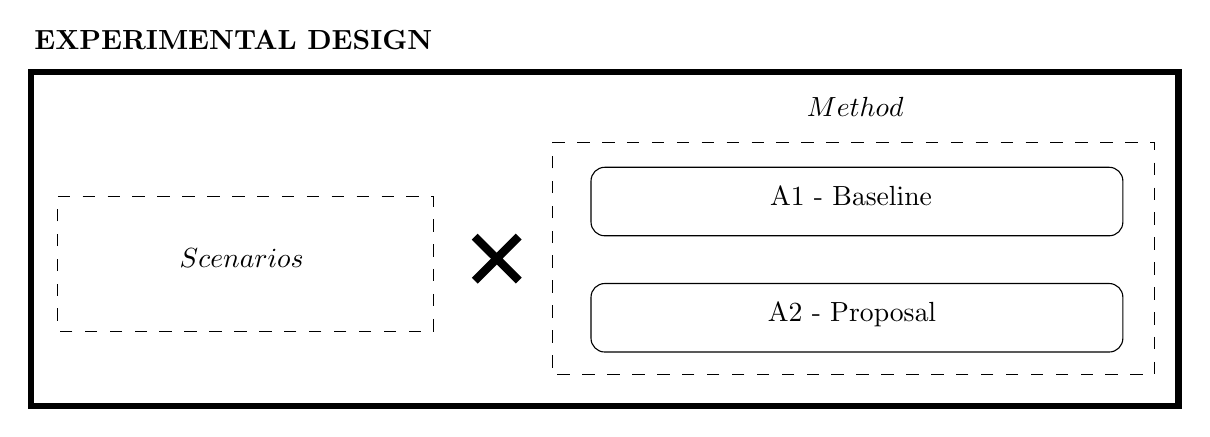
\begin{tikzpicture}[x=0.75pt,y=0.75pt,yscale=-1,xscale=1]
%uncomment if require: \path (0,201); %set diagram left start at 0, and has height of 201

%Rounded Rect [id:dp06575569211056953] 
\draw   (279.42,79.6) .. controls (279.42,75.95) and (282.37,73) .. (286.02,73) -- (529.06,73) .. controls (532.7,73) and (535.66,75.95) .. (535.66,79.6) -- (535.66,99.4) .. controls (535.66,103.05) and (532.7,106) .. (529.06,106) -- (286.02,106) .. controls (282.37,106) and (279.42,103.05) .. (279.42,99.4) -- cycle ;
%Shape: Rectangle [id:dp6932811140385843] 
\draw  [dash pattern={on 4.5pt off 4.5pt}] (22.5,87) -- (203.5,87) -- (203.5,152) -- (22.5,152) -- cycle ;
%Shape: Rectangle [id:dp9822494345299366] 
\draw  [dash pattern={on 4.5pt off 4.5pt}] (260.75,61) -- (551,61) -- (551,173) -- (260.75,173) -- cycle ;
%Shape: Rectangle [id:dp3952140034216508] 
\draw  [line width=2.25]  (9.5,27) -- (562.5,27) -- (562.5,188) -- (9.5,188) -- cycle ;
\draw  [line width=3]  (223.37,106.42) -- (244.63,127.58)(244.58,106.37) -- (223.42,127.63) ;
%Rounded Rect [id:dp9781270849297624] 
\draw   (279.42,135.6) .. controls (279.42,131.95) and (282.37,129) .. (286.02,129) -- (529.06,129) .. controls (532.7,129) and (535.66,131.95) .. (535.66,135.6) -- (535.66,155.4) .. controls (535.66,159.05) and (532.7,162) .. (529.06,162) -- (286.02,162) .. controls (282.37,162) and (279.42,159.05) .. (279.42,155.4) -- cycle ;

% Text Node
\draw (80,111) node [anchor=north west][inner sep=0.75pt]    {$Scenarios$};
% Text Node
\draw (382.17,38) node [anchor=north west][inner sep=0.75pt]    {$Method$};
% Text Node
\draw (10,6) node [anchor=north west][inner sep=0.75pt]   [align=left] {\textbf{EXPERIMENTAL DESIGN}};
% Text Node
\draw (364.41,81) node [anchor=north west][inner sep=0.75pt]   [align=left] {A1 - Baseline};
% Text Node
\draw (363.41,137) node [anchor=north west][inner sep=0.75pt]   [align=left] {A2 - Proposal};


\end{tikzpicture}}
    \caption{Experimental setup with the treatments performed by the simulator}
    \label{fig:exp_setup}
\end{figure}

All scenarios created from the variables' values definition consider the same size of members' set $|E|=5$, the mission size $|M|=30$, and an initial C2 Approach $\omega_0 =$ De-Conflicted. Finally, each simulation scenario has a deadline of 1000 ticks of execution time.


%The simulation uses a set of random variables to define some elements during execution, i.e., UAVs, and tasks position, and sensor that will be affected by the context event. For a consistent comparison between the methods A1 and A2, the same set of random variables is used by both methods during the same execution number.

%%%%%%%%%%%%%%%%%%%%%%%%%%%%%%%%%%
% SUBSECTION 
%%%%%%%%%%%%%%%%%%%%%%%%%%%%%%%%%%
\subsection{Results and Analysis}

Table~\ref{table:results02} shows the results obtained by the simulation with the scenarios described in Section~\ref{sub:scenarios}. Figures~\ref{fig:m1},~\ref{fig:m2}, and~\ref{fig:m3} make a graphical comparison that shows a statistical difference among results obtained with the A1 and A2 treatments. Figure~\ref{fig:m1} confirms the maneuvering presence in all scenarios with the A2 treatment. The results are constant value due to the cost in terms of time to perform a C2 Approach change. As expected, the A1 method does not involve such behavior due to the nonexistence of C2 Maneuver Agility.

\begin{figure}[ht]
\centering
\begin{minipage}{.5\textwidth}
    \centering
    \small
    \fontsize{7}{7}\selectfont
	\captionof{table}{Metrics results}
    \label{table:results02}
    \begin{tabular}{rrrr} \hline
		& \bf{M1}
        & \bf{M2}
		& \bf{M3} \\  \hline 
		
		& Mean(St.Dev.)  & Mean(St.Dev.) & Mean(St.Dev.)\\ [1ex]
		
		\multicolumn{3}{l}{\textbf{$\longrightarrow$ Scenario 1 }} \\
	% Scenario  1 
\bf{A1}  & 0.0 ($\pm$0.0)  & 890.0 ($\pm$66.8)  & 82.0 ($\pm$5.9)  \\
\bf{A2}  & 1.7 ($\pm$0.3)  & 945.5 ($\pm$33.1)  & 97.7 ($\pm$2.9)  \\ [1ex]
	
	\multicolumn{3}{l}{\textbf{$\longrightarrow$ Scenario 2 }} \\
% Scenario  2 
\bf{A1}  & 0.0 ($\pm$0.0)  & 866.5 ($\pm$72.3)  & 77.5 ($\pm$6.3) \\
\bf{A2}  & 2.6 ($\pm$0.6)  & 934.0 ($\pm$33.0)  & 95.2 ($\pm$4.2) \\ [1ex]
	
	\multicolumn{3}{l}{\textbf{$\longrightarrow$ Scenario 3 }} \\
% Scenario  3 
\bf{A1}  & 0.0 ($\pm$0.0)  & 782.1 ($\pm$78.3)  & 63.7 ($\pm$5.5) \\
\bf{A2}  & 2.8 ($\pm$0.3)  & 883.0 ($\pm$49.2)  & 69.1 ($\pm$4.5) \\ [1ex]
	
	\multicolumn{3}{l}{\textbf{$\longrightarrow$ Scenario 4 }} \\
% Scenario  4 
\bf{A1}  & 0.0 ($\pm$0.0)  & 799.1 ($\pm$77.0)  & 63.6 ($\pm$5.3) \\
\bf{A2}  & 3.0 ($\pm$0.1)  & 913.4 ($\pm$35.9)  & 84.5 ($\pm$5.1) \\ [1ex]
	
	\multicolumn{3}{l}{\textbf{$\longrightarrow$ Scenario 5 }} \\
% Scenario  5 
\bf{A1}  & 0.0 ($\pm$0.0)  & 733.7 ($\pm$75.5)  & 54.6 ($\pm$4.6)  \\
\bf{A2}  & 2.9 ($\pm$0.2)  & 887.7 ($\pm$48.4)  & 70.7 ($\pm$5.1) \\ [1ex]
	
	\multicolumn{3}{l}{\textbf{$\longrightarrow$ Scenario 6 }} \\
% Scenario  6 
\bf{A1}  & 0.0 ($\pm$0.0)  & 700.6 ($\pm$79.4)  & 42.0 ($\pm$4.5) \\
\bf{A2}  & 2.9 ($\pm$0.2)  & 910.5 ($\pm$59.3)  & 65.7 ($\pm$5.9) \\ [1ex]
	
	\multicolumn{3}{l}{\textbf{$\longrightarrow$ Scenario 7 }} \\
% Scenario  7 
\bf{A1}  & 0.0 ($\pm$0.0)  & 686.2 ($\pm$58.4)  & 41.1 ($\pm$3.5)  \\
\bf{A2}  & 2.8 ($\pm$0.3)  & 820.5 ($\pm$61.4)  & 60.1 ($\pm$5.6)  \\ [1ex]
	
	\multicolumn{3}{l}{\textbf{$\longrightarrow$ Scenario 8 }} \\
% Scenario  8 
\bf{A1}  & 0.0 ($\pm$0.0)  & 629.7 ($\pm$68.6)  & 36.3 ($\pm$3.8) \\
\bf{A2}  & 2.8 ($\pm$0.3)  & 785.1 ($\pm$58.3)  & 52.1 ($\pm$4.7) \\ [1ex]
	
	\multicolumn{3}{l}{\textbf{$\longrightarrow$ Scenario 9 }} \\
% Scenario  9 
\bf{A1}  & 0.0 ($\pm$0.0)  & 491.0 ($\pm$74.2)  & 26.4 ($\pm$3.7) \\
\bf{A2}  & 3.0 ($\pm$0.1)  & 743.2 ($\pm$66.1)  & 53.2 ($\pm$5.1) \\ [1ex]
	
	\multicolumn{3}{l}{\textbf{$\longrightarrow$ Scenario 10 }} \\
		
% Scenario  10 
\bf{A1}  & 0.0 ($\pm$0.0)  & 393.4 ($\pm$81.2)  & 24.3 ($\pm$2.6) \\
\bf{A2}  & 2.9 ($\pm$0.2)  & 650.7 ($\pm$114.8)  & 38.8 ($\pm$4.7) \\ [1ex]
		\hline
	\end{tabular}
\end{minipage}%
\begin{minipage}{.5\textwidth}
  \centering
  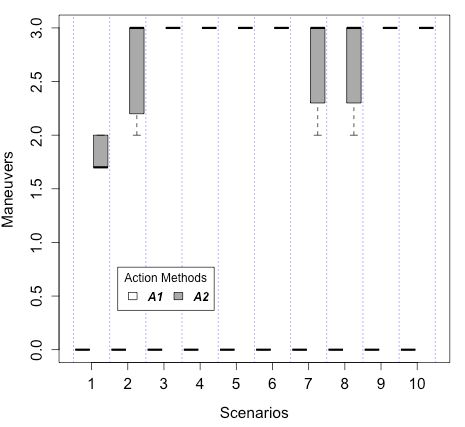
\includegraphics[width=0.95\linewidth]{figures/graphs/Boxplot_M2.png}
  \captionof{figure}{Total of maneuverings (M1)}
  \label{fig:m1}
\end{minipage}
\end{figure}

\begin{figure}
\centering
\begin{minipage}{.5\textwidth}
  \centering
  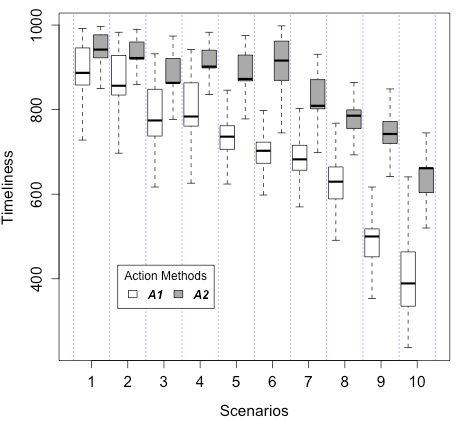
\includegraphics[width=0.95\linewidth]{figures/graphs/Boxplot_M3.png}
  \captionof{figure}{Total operation time (M2)}
  \label{fig:m2}
\end{minipage}%
\begin{minipage}{.5\textwidth}
  \centering
  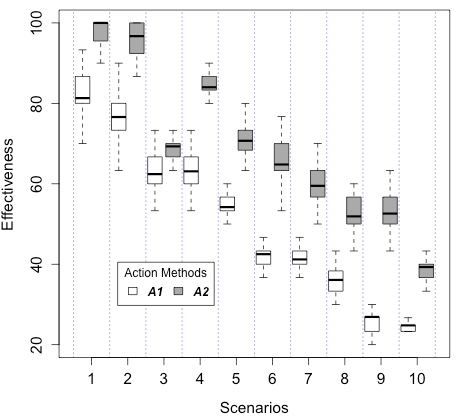
\includegraphics[width=0.95\linewidth]{figures/graphs/Boxplot_M5.png}
  \captionof{figure}{Completed tasks (M3)}
  \label{fig:m3}
\end{minipage}
\end{figure}

Similar analysis can be applied to M1 and M2 metrics. Figure~\ref{fig:m2} shows significant difference among the time in operation, i.e., timeliness, of the methods A1 and A2. Complex scenarios with more events causing context changes, the system with C2 Agility keeps running for longer. In a such condition, the awareness obtained by the system through the C2 Approach selected becomes the system more suitable to deal with a new circumstance and capable to keep engaged in the mission. In addition, the metric M3 (Figure~\ref{fig:m3}) shows a better mission completeness when the system makes coordination and adaptation adjustments in runtime in face of context changes. 

More time consumed by the system could be related to the cost in terms of time to perform such maneuvers. However, A combined analysis of the results showed in Figures~\ref{fig:m2} and ~\ref{fig:m3}, indicates a capacity to keep running under context perturbations and performing the mission tasks. It gives more resilience to the system achieving C2 Agility and, consequently, C2 Maneuver Agility. Although sensor reconfigurations are happening in all scenarios due to C2 Agility implemented, those with higher count of maneuvers values (M1) pointed out better results (M3) when compared with the A1 method. This aspect shows evidence of gains from the incorporation of C2 Maneuver agility in the implementation.

As the system gets different information sharing level through C2 Approach changes, i.e., maneuverings, it can adapt itself according to the different conditions that occur in a dynamic scenario. The Figure~\ref{fig:m3} shows that the capacity of the C2 system to solve tasks, under the effect of changes in the context that alter its functioning, is more significant in the A2 method where C2 Maneuver Agility provides the system awareness modification. In turn, the static nature of the A1 method limits its performance since the initial configuration is the only and unique option to execute the mission.

All results obtained in our experiment were submitted to a Shapiro-Wilk test~\citep{stat001}. Such a test gave us a \textit{p-value} less than 0.05 and it indicates a non-normal distribution. Based on this, we applied a Mann-Whitney U Test~\citep{stat002}, available in R tool as Wilcoxon-test, to check statistical differences among the samples of each action method applied. The statistical analysis confirmed the difference between all results from A1 and A2 methods, collected in all scenarios simulated.


% In summary, the empirical findings indicate a better overall performance using the A2 method that implements C2 Agility. This capability is only completed with the C2 Maneuver Agility concept, where the system looks for a suitable coordination structure, i.e., C2 Approach, to deal with context changes. Results show a relation between the number of C2 Approach changes and the number of completed tasks, indicating its contribution to keeping the system engaged with the mission. These maneuverings, i.e., C2 Approach changes, have a cost in terms of time, and even with this, the time in operation, i.e., M2 metric, increases along with the mission completeness(M3). Besides, the model(CS) used to represent the entities' behavior that makes up the system, through the use of roles, proved to be effective in guiding the implementation of the simulator. The capabilities embedded in the system result in a resilience increasing and enable the behavioral model the ability to cope with context changes and perturbations in dynamic scenarios.

In summary, the empirical findings indicate a better overall performance using the A2 method that implements C2 Agility. This capability was achievable with the presence of the C2 Maneuver Agility concept, where the system looks for a suitable coordination structure, i.e., C2 Approach, to deal with context changes. Results show a relation between the number of C2 Approach changes and the number of completed tasks, that may indicate a contribution of maneuvering to keeping the system engaged with the mission. These maneuverings, i.e., C2 Approach changes, have a cost in terms of time, and even with this, the time in operation, i.e., M2 metric, increases along with the mission completeness (M3). Besides, the proposed communication model (CS) along side with the adoption of roles (PG) used to represent the entities' behavior proved to be effective in guiding the implementation of the simulator. The capabilities embedded in the system result in a resilience increasing and enable the behavioral model the ability to cope with context changes and perturbations in dynamic scenarios.


%<<< 
%PRECISAMOS ADICIONAR: 
% -> o modelo comportamental (CS) pôde representar a coordenação entre os papeis que modelam o cenário de C2 -> missing
% -> O C2 Maneuver Agility compõe a definição de C2 Agility e sua implementação possibilita a adequada troca de informações em busca da awareness do sistema, de modo que ele se adeque aos diversos contextos (Não precisamos falar de configuração dos elementos) -> +/-
% -> evidencias -> accomplished
%>>>